\chapter[RESULTADOS]{RESULTADOS}

\section{Malha em formato 'L'}
Conforme já especificado, a malha a ser resolvida para o problema de difusão de calor 2D é uma malha em formato 'L'. Tal malha, gerada por uma triangulação de Delaunay em um domínio fechado é apresentada na figura \ref{fig:malha-inicial}.

Nessa malha aparecem em todos as células o valor da solução analítica seguido do valor numérico encontrado. Em vermelho estão os centroides dos volumes 'Reais' e em azul o centroide dos volumes 'Virtuais'

Além de visualizar a malha, é muito útil a informação de maior ângulo, menor ângulo, desvio padrão do ângulo, média da qualidade da malha, maior qualidade, menor qualidade resultando nas tabelas \ref{tab:angulos-malha-inicial} e \ref{tab:qualidades-malha-inicial}. As qualidades se referem às qualidades de cada volume que constitui a malha, sendo que esta é obtida pela fórmula:

\begin{equation}
    2 \frac{r}{R}
\end{equation}

Onde $r$ é o raio da circunferência inscrita e $R$ é o raio da circunferência circunscrita.
\criarsimbolo{$r$}{raio daa circunferência inscrita}
\criarsimbolo{$R$}{raio daa circunferência circunscrita}

A média das qualidades pode ser associada à malha como uma indicação da sua qualidade geral.

De modo a testar os algoritmos de suavização da malha, esta malha inicial foi distorcida, ou seja, seus vértices internos foram propositalmente alterados de posição, resultando na malha \ref{fig:malha-ruim} com as tabelas \ref{tab:angulos-malha-distorcida} e \ref{tab:qualidades-malha-distorcida}.

\newpage
\subsection{Malha Inicial}

\begin{figure}[ht]
    \centering
    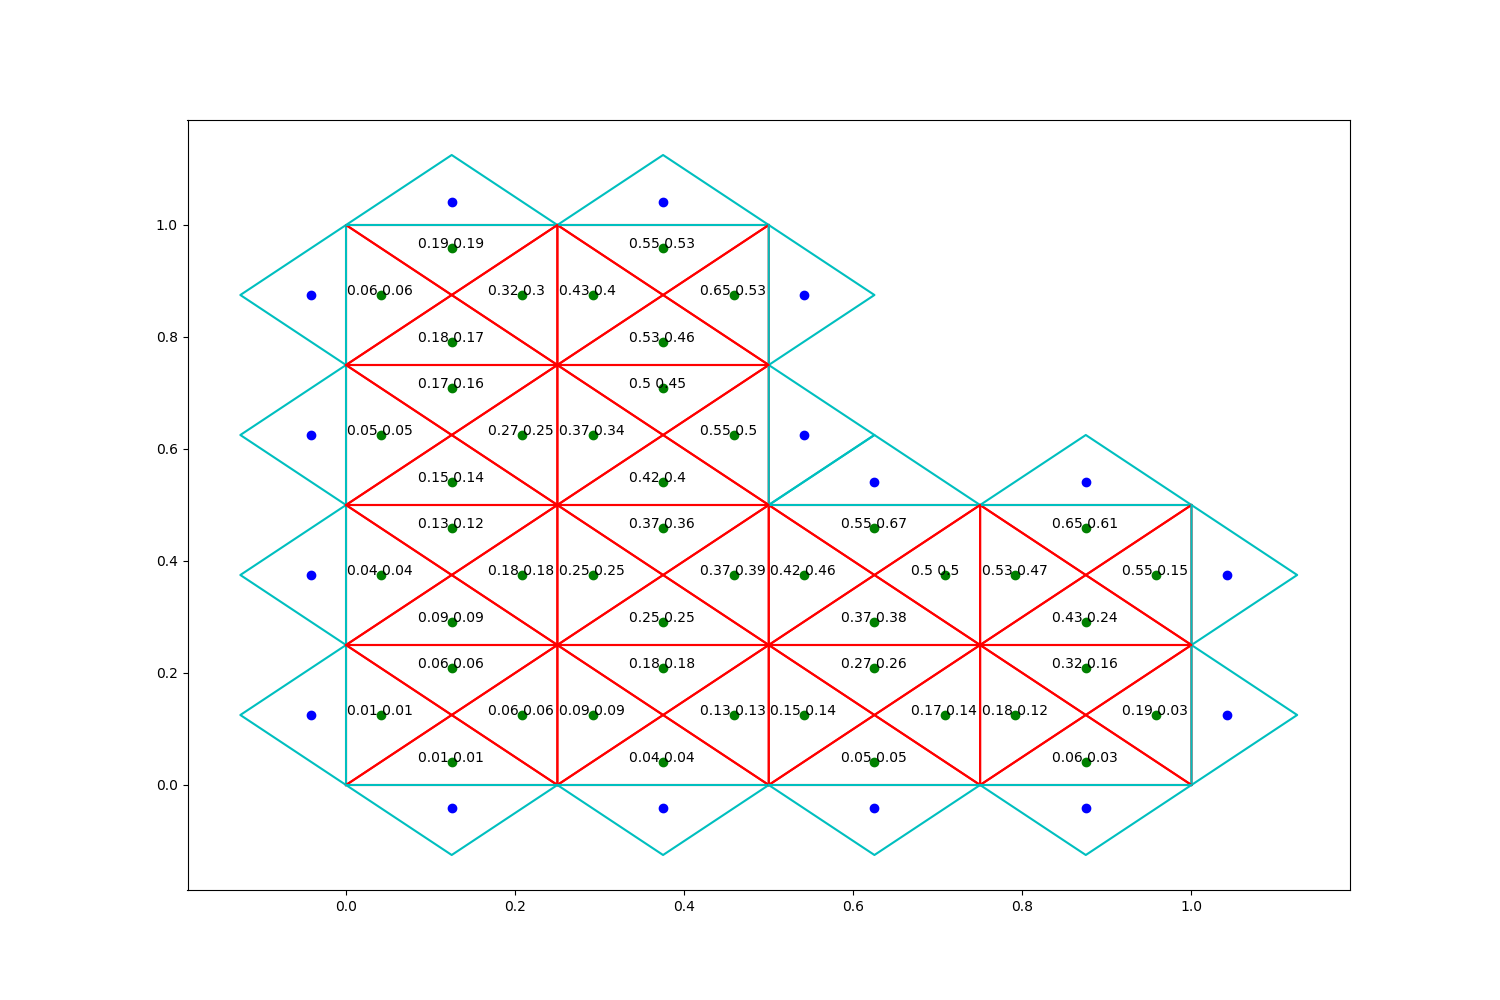
\includegraphics[width=1\linewidth]{fig/malha_inicial.png}
    \caption{Malha Inicial}
    \label{fig:malha-inicial}
\end{figure}

\begin{table}[hb]
 \centering
 \par\caption{Ângulos da Malha Inicial}
\begin{tabular}{c|c|c|c}
 Maior&menor&média&desvio padrão\\\hline\hline
  90&45&60&21.268663\\\hline
 \end{tabular}
 \label{tab:angulos-malha-inicial}
\end{table}

\begin{table}[hb]
 \centering
 \par\caption{Qualidades da Malha Inicial}
\begin{tabular}{c|c|c|c}
 Maior&menor&média&desvio padrão\\\hline\hline
 8.284271e-01&8.284271e-01&8.284271e-01&0\\\hline
 \end{tabular}
 \label{tab:qualidades-malha-inicial}
\end{table}

\newpage
\subsection{Malha Distorcida}

\begin{figure}[ht]
    \centering
    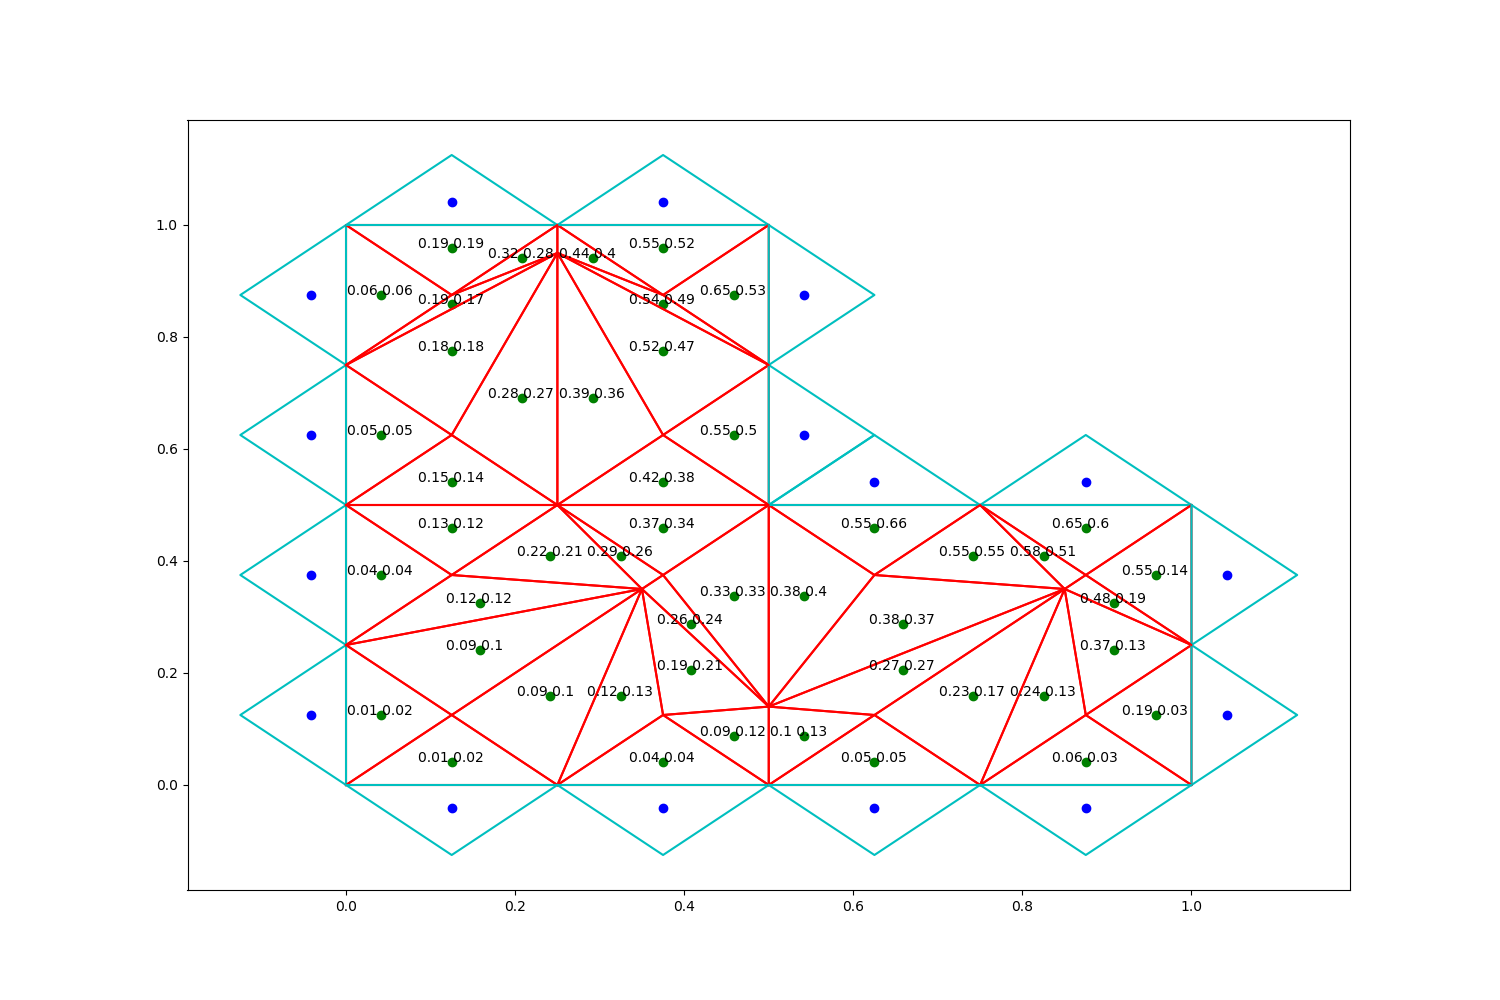
\includegraphics[width=1\linewidth]{fig/malha-ruim.png}
    \caption{Malha Inicial após Deformações}
    \label{fig:malha-ruim}
\end{figure}

\begin{table}[hb]
\centering
\par\caption{Ângulos da Malha Distorcida}
\begin{tabular}{c|c|c|c}
Maior&menor&média&desvio padrão\\\hline\hline
165.963757&6.340192&60.000000&30.017315\\\hline
\end{tabular}
\label{tab:angulos-malha-distorcida}
\end{table}

\begin{table}[hb]
\centering
\par\caption{Qualidades da Malha Distorcida}
\begin{tabular}{c|c|c|c}
Maior&menor&média&desvio padrão\\\hline\hline
0.928007&0.029467&0.700351&0.227835\\\hline
\end{tabular}
\label{tab:qualidades-malha-distorcida}
\end{table}

\newpage
\subsection{Centroidal Path Tesselation}

Em seguida, executou-se os algoritmos de melhoramento da malha com apenas uma iteração, começando pelo método centroidal patch tesselation (CPT) como na figura \ref{fig:malha-cpt}

\begin{figure}[ht]
    \centering
    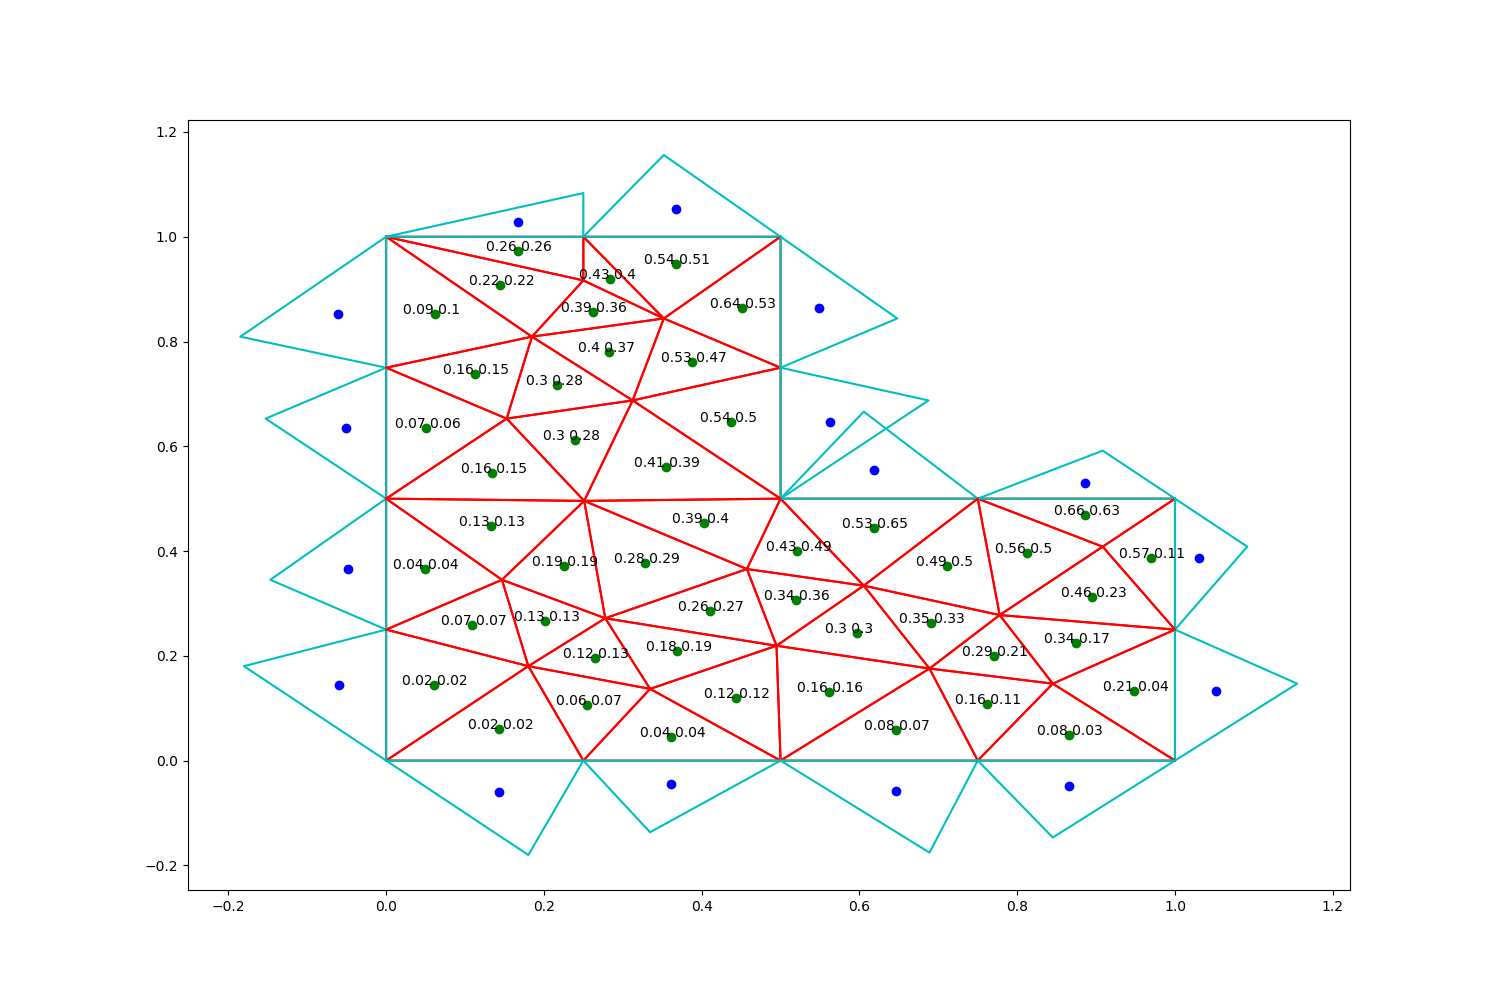
\includegraphics[width=1\linewidth]{fig/malha-cpt.png}
    \caption{Melhoramento CPT}
    \label{fig:malha-cpt}
\end{figure}

\begin{table}[hb]
\centering
\par\caption{Ângulos da Malha CPT}
\begin{tabular}{c|c|c|c}
Maior&menor&média&desvio padrão\\\hline\hline
125.476562&18.434949&60.000000&16.412226\\\hline
\end{tabular}
\label{tab:angulos-malha-cpt}
\end{table}

\begin{table}[hb]
\centering
\par\caption{Qualidades da Malha CPT}
\begin{tabular}{c|c|c|c}
Maior&menor&média&desvio padrão\\\hline\hline
0.997240&0.376030&0.889689&0.126673\\\hline
\end{tabular}
\label{tab:qualidades-malha-cpt}
\end{table}

\newpage
\subsection{Optimal Delaunay Tesselation}

\begin{figure}[ht]
    \centering
    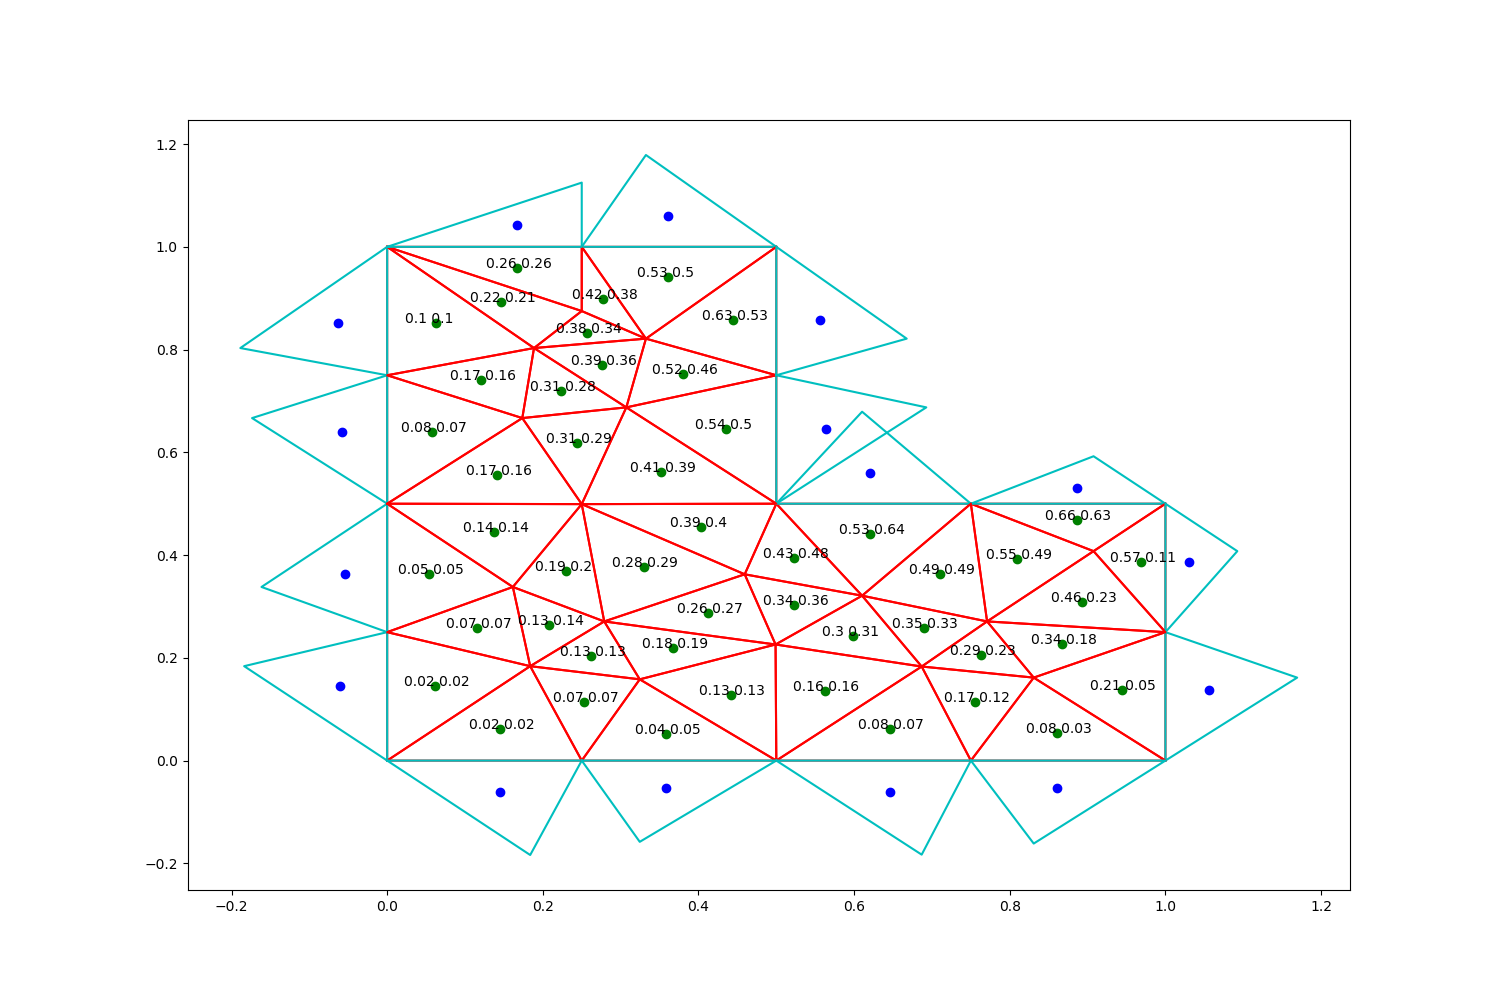
\includegraphics[width=1\linewidth]{fig/malha-odt.png}
    \caption{Melhoramento ODT}
    \label{fig:malha-odt}
\end{figure}

\begin{table}[hb]
\centering
\par\caption{Ângulos da Malha ODT}
\begin{tabular}{c|c|c|c}
Maior&menor&média&desvio padrão\\\hline\hline
123.086976&19.672726&60.000000&16.668335\\\hline
\end{tabular}
\label{tab:angulos-malha-odt}
\end{table}

\begin{table}[hb]
\centering
\par\caption{Qualidades da Malha ODT}
\begin{tabular}{c|c|c|c}
Maior&menor&média&desvio padrão\\\hline\hline
0.992361&0.417613&0.885554&0.119807\\\hline
\end{tabular}
\label{tab:qualidades-malha-odt}
\end{table}

\newpage
\subsection{Centroidal Voronoi Tesselation}

\begin{figure}[ht]
    \centering
    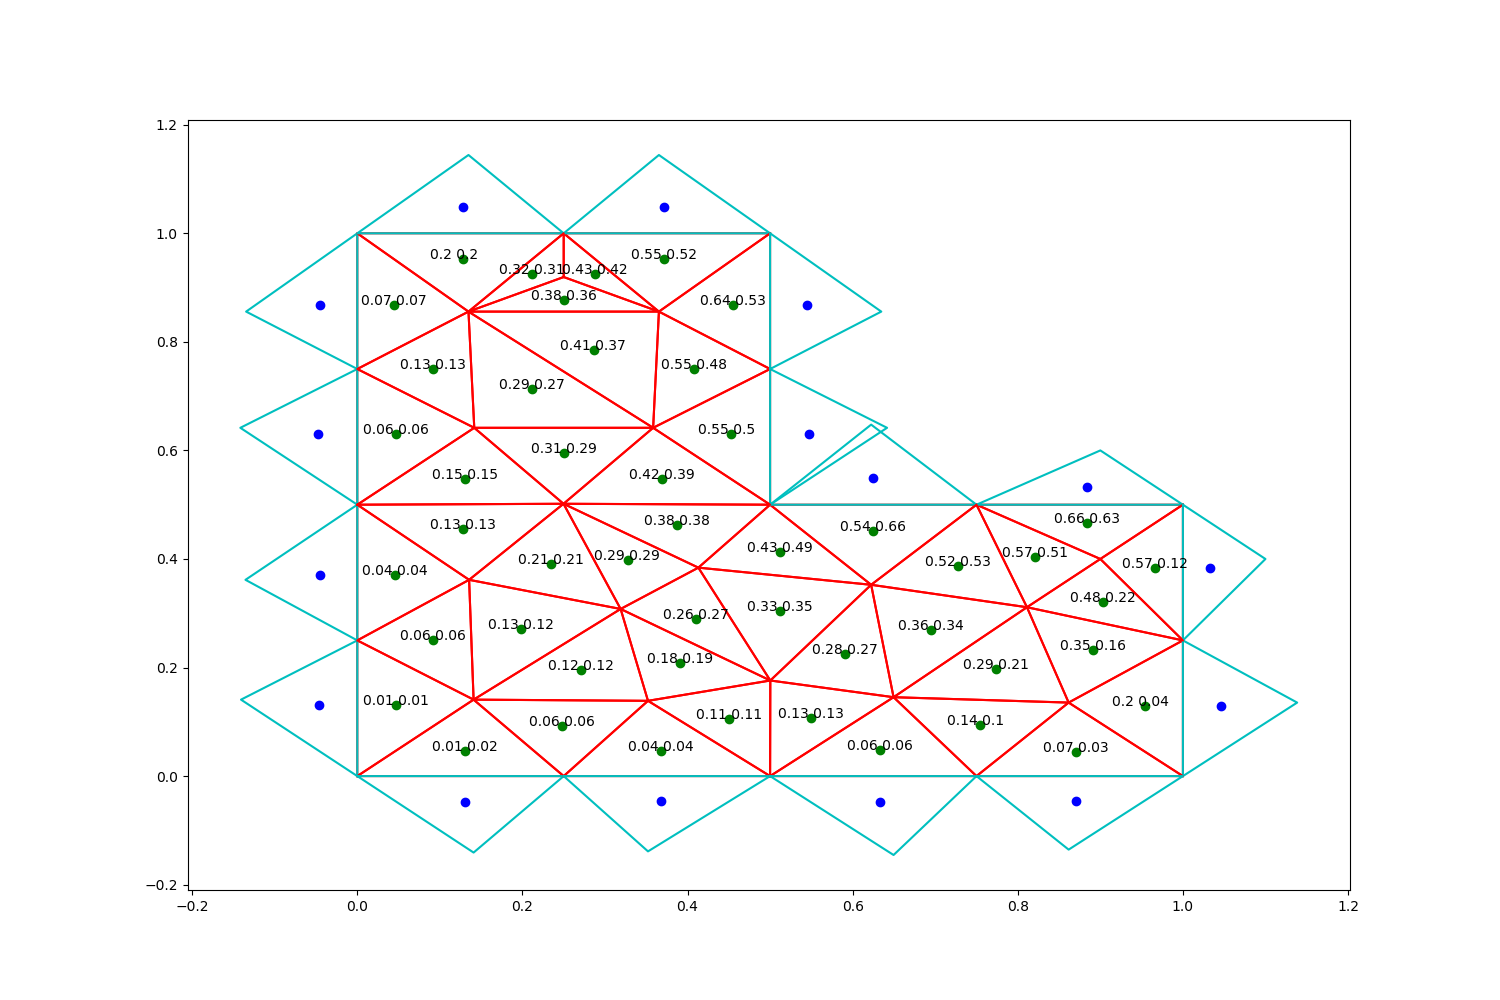
\includegraphics[width=1\linewidth]{fig/malha-cvt.png}
    \caption{Melhoramento CVT}
    \label{fig:malha-cvt}
\end{figure}

\begin{table}[hb]
\centering
\par\caption{Ângulos da Malha CVT}
\begin{tabular}{c|c|c|c}
Maior&menor&média&desvio padrão\\\hline\hline
122.171970&22.444618&60.000000&18.811931\\\hline
\end{tabular}
\label{tab:angulos-malha-cvt}
\end{table}

\begin{table}[hb]
\centering
\par\caption{Qualidades da Malha CVT}
\begin{tabular}{c|c|c|c}
Maior&menor&média&desvio padrão\\\hline\hline
0.999421&0.436461&0.865904&0.116918\\\hline
\end{tabular}
\label{tab:qualidades-malha-cvt}
\end{table}

\newpage
\subsection{Angle Based Tesselation}

\begin{figure}[ht]
    \centering
    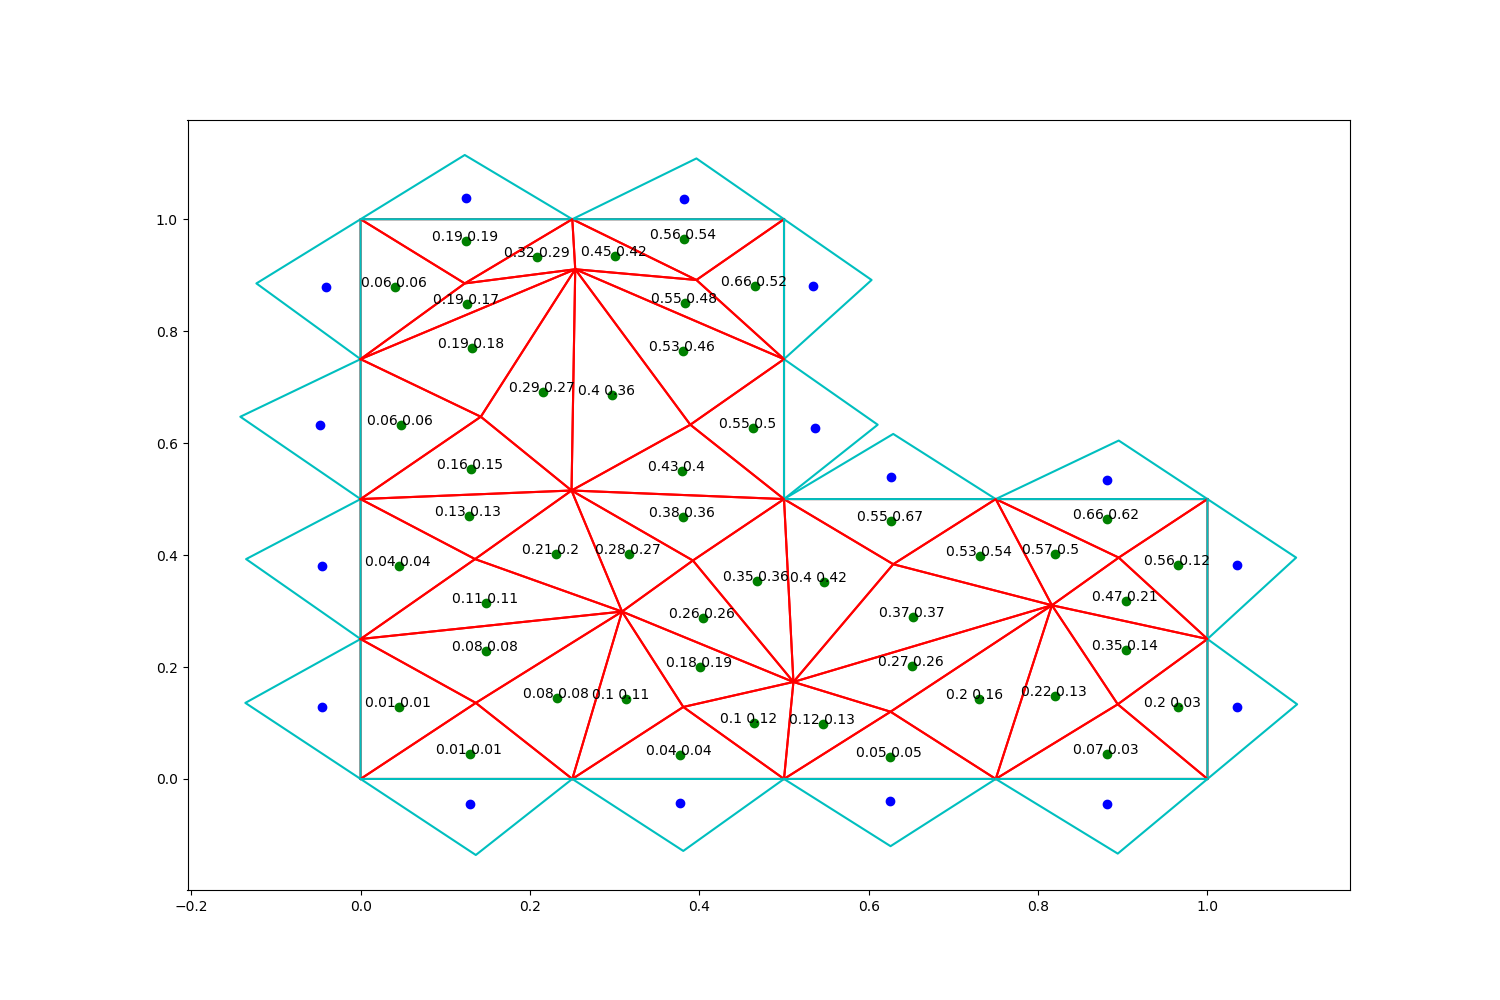
\includegraphics[width=1\linewidth]{fig/malha-angulos.png}
    \caption{Melhoramento Ângulos}
    \label{fig:malha-angulos}
\end{figure}

\begin{table}[hb]
\centering
\par\caption{Ângulos da Malha Ângulos}
\begin{tabular}{c|c|c|c}
Maior&menor&média&desvio padrão\\\hline\hline
143.247344&15.367140&60.000000&26.037994\\\hline
\end{tabular}
\label{tab:angulos-malha-angulos}
\end{table}

\begin{table}[hb]
\centering
\par\caption{Qualidades da Malha Ângulos}
\begin{tabular}{c|c|c|c}
Maior&menor&média&desvio padrão\\\hline\hline
0.972793&0.188339&0.758870&0.141551\\\hline
\end{tabular}
\label{tab:qualidades-malha-angulos}
\end{table}

\newpage
\subsection{Gurobi Optimization Based Tesselation}

\begin{figure}[ht]
    \centering
    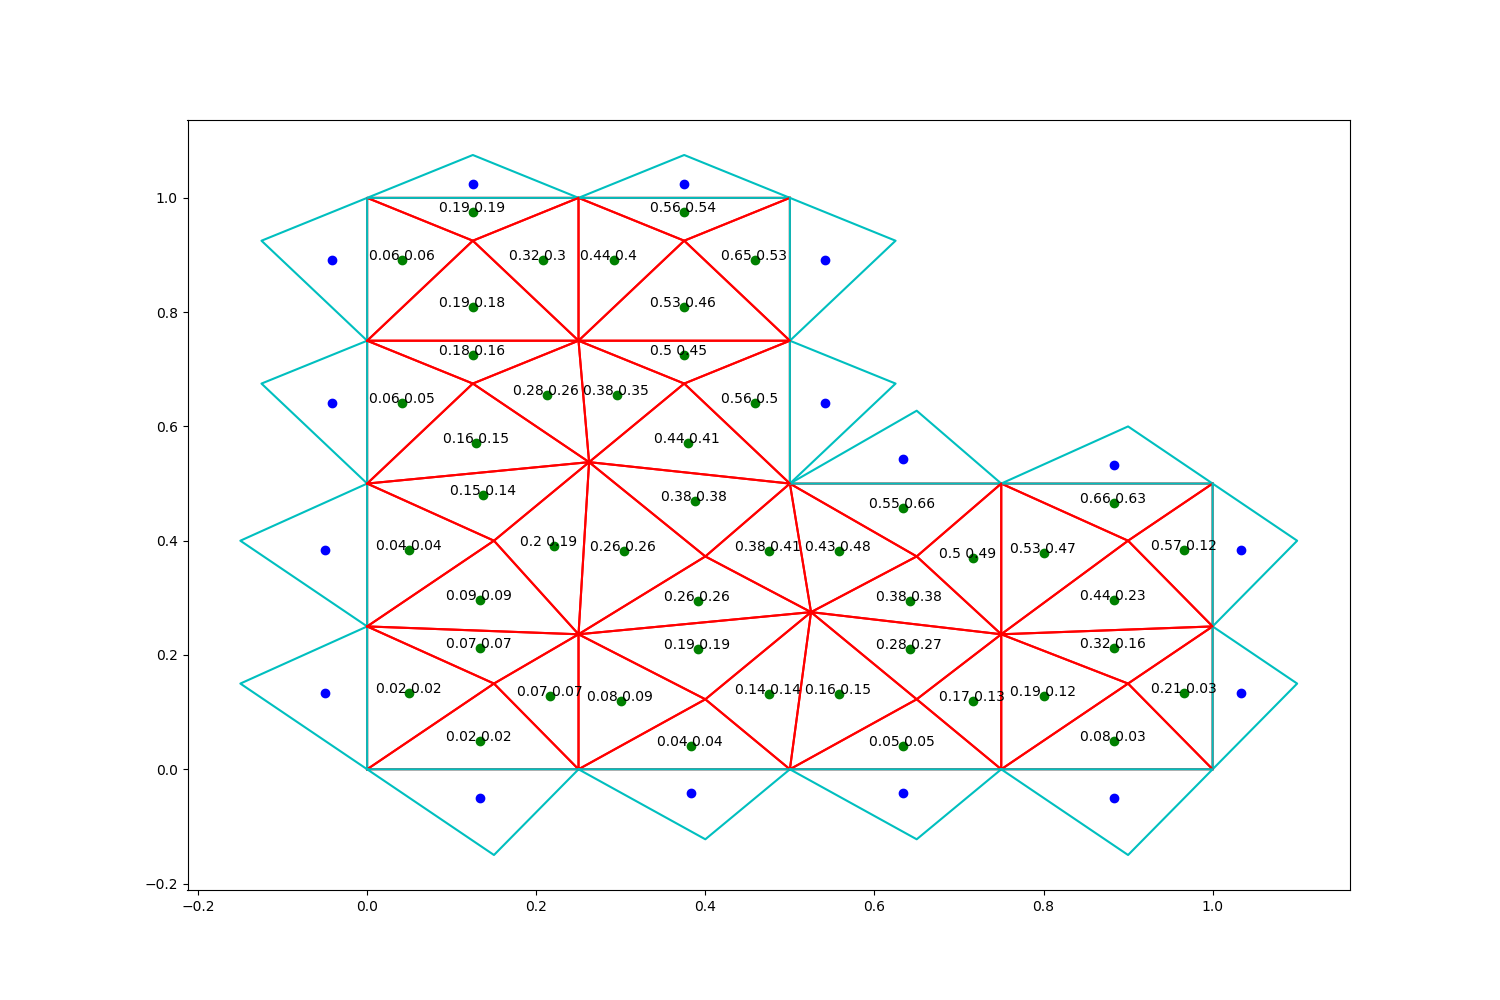
\includegraphics[width=1\linewidth]{fig/malha-gurobi.png}
    \caption{Melhoramento Gurobi}
    \label{fig:malha-gurobi}
\end{figure}

\begin{table}[hb]
\centering
\par\caption{Ângulos da Malha Gurobi}
\begin{tabular}{c|c|c|c}
Maior&menor&média&desvio padrão\\\hline\hline
118.072487&30.541971&60.000000&24.045397\\\hline
\end{tabular}
\label{tab:angulos-malha-gurobi}
\end{table}

\begin{table}[hb]
\centering
\par\caption{Qualidades da Malha Gurobi}
\begin{tabular}{c|c|c|c}
Maior&menor&média&desvio padrão\\\hline\hline
0.973601&0.488795&0.790714&0.134577\\\hline
\end{tabular}
\label{tab:qualidades-malha-gurobi}
\end{table}

\newpage
\subsection{Genetic Algorithm Based Tesselation}

\begin{figure}[ht]
    \centering
    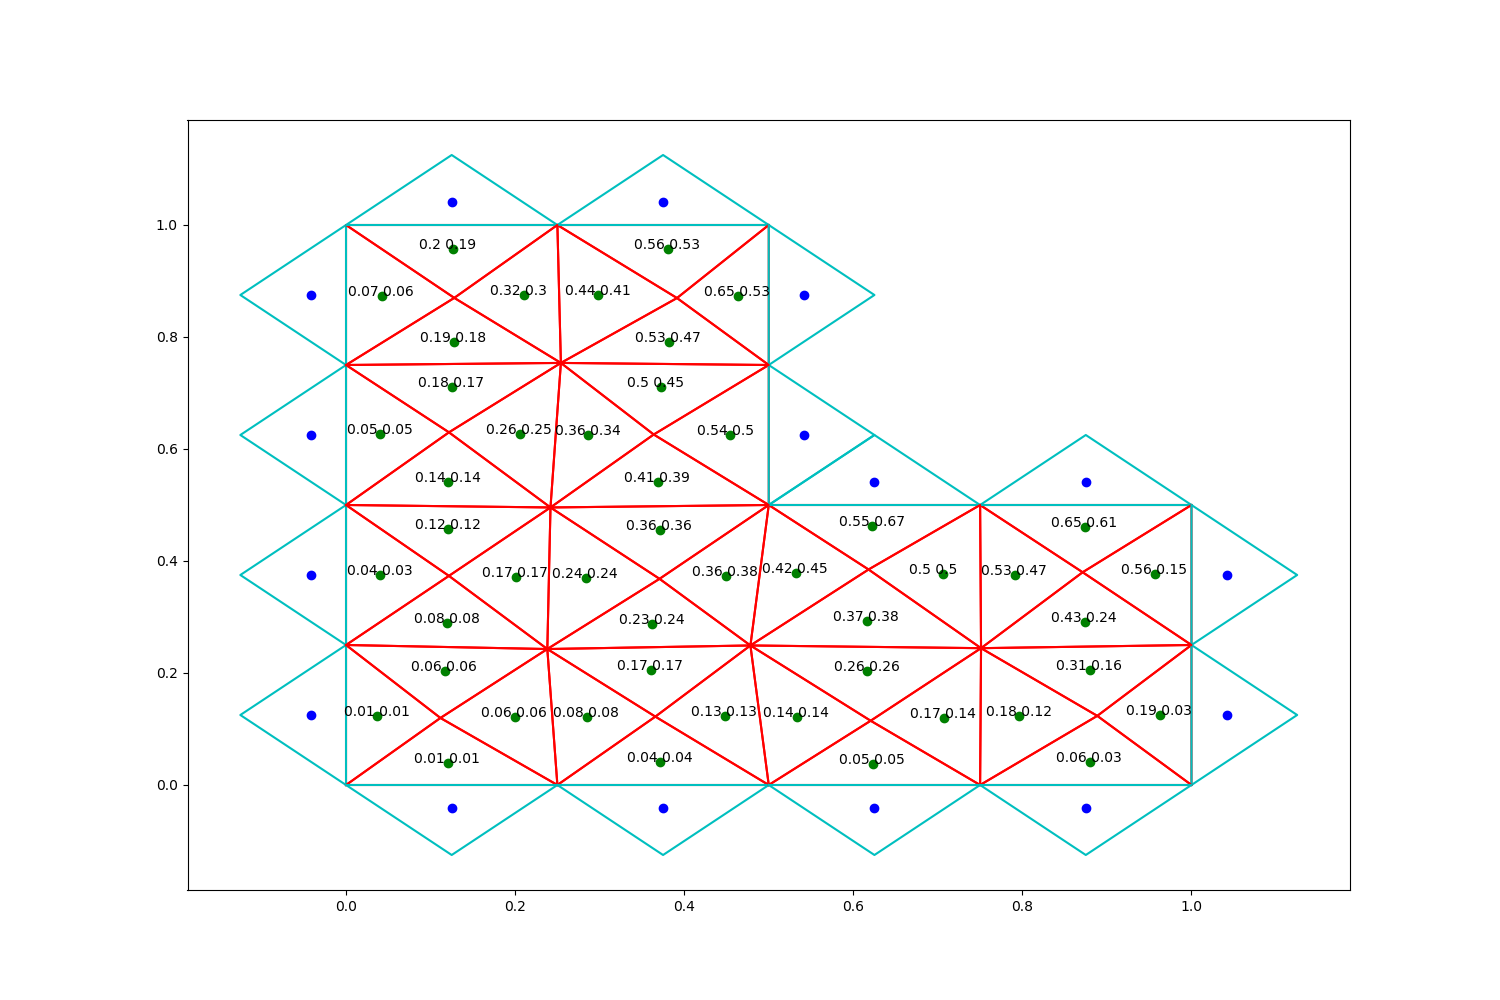
\includegraphics[width=1\linewidth]{fig/malha-ga.png}
    \caption{Melhoramento GA}
    \label{fig:malha-ga}
\end{figure}

\begin{table}[hb]
\centering
\par\caption{Ângulos da Malha GA}
\begin{tabular}{c|c|c|c}
Maior&menor&média&desvio padrão\\\hline\hline
100.102771&35.502815&60.000000&21.548683\\\hline
\end{tabular}
\label{tab:angulos-malha-ga}
\end{table}

\begin{table}[hb]
\centering
\par\caption{Qualidades da Malha GA}
\begin{tabular}{c|c|c|c}
Maior&menor&média&desvio padrão\\\hline\hline
0.915087&0.715044&0.824170&0.041392\\\hline
\end{tabular}
\label{tab:qualidades-malha-ga}
\end{table}